\documentclass{beamer}

% Theme setup
\usetheme{Madrid}
\usecolortheme{default}
\setbeamertemplate{navigation symbols}{}
\setbeamertemplate{footline}[frame number]

% Packages
% \usepackage[utf8]{inputenc}
\usepackage{graphicx}
\usepackage{hyperref}
\usepackage{lmodern}
\usepackage{listings}
\lstset{
    basicstyle = \ttfamily\scriptsize,
    breaklines = true,
    breakatwhitespace = false,
    columns = fullflexible,
    keepspaces = true,
    showstringspaces = false,
    frame = single
}

% Title info
\title{\textbf{RRT or Rapidly-exploring Random Tree \\ (wheeled robots, RRT, Prim's algorithm \& MST, path and motion planning for solving mazes)}}
\subtitle{\textit{Robotic Systems I}}
\author{
    Konstantinos Asimakopoulos \hspace{2em} \textit{k\_asimakopoulos@ac.upatras.gr}
    Lampros Printzios \hspace{2em} \textit{printzios\_lampros@ac.upatras.gr}
}
\institute{Department of Electrical and Computer Engineering \\ University of Patras}
\date{March 2, 2026}

\begin{document}

% Title Slide
\begin{frame}
    \titlepage
\end{frame}

% Slide: Table of Contents
\begin{frame}{Table of Contents}
    \begin{columns}[T]
        \begin{column}{0.45\textwidth}
            \tableofcontents[sections={-3}]
        \end{column}
        \begin{column}{0.45\textwidth}
            \tableofcontents[sections={4-}]
        \end{column}
    \end{columns}
\end{frame}

% Differential Drive Robot (DDR)
\section{Differential Drive Robot (DDR)}
\begin{frame}
    \frametitle{\insertsection}
    Typical DDRs are TurtleBot3 Waffle Pi (used in this lab) and TurtleBot3 Burger, that are showed below.
    \vspace{10pt}
    \begin{columns}
        \begin{column}{0.55\linewidth}
            \centering
            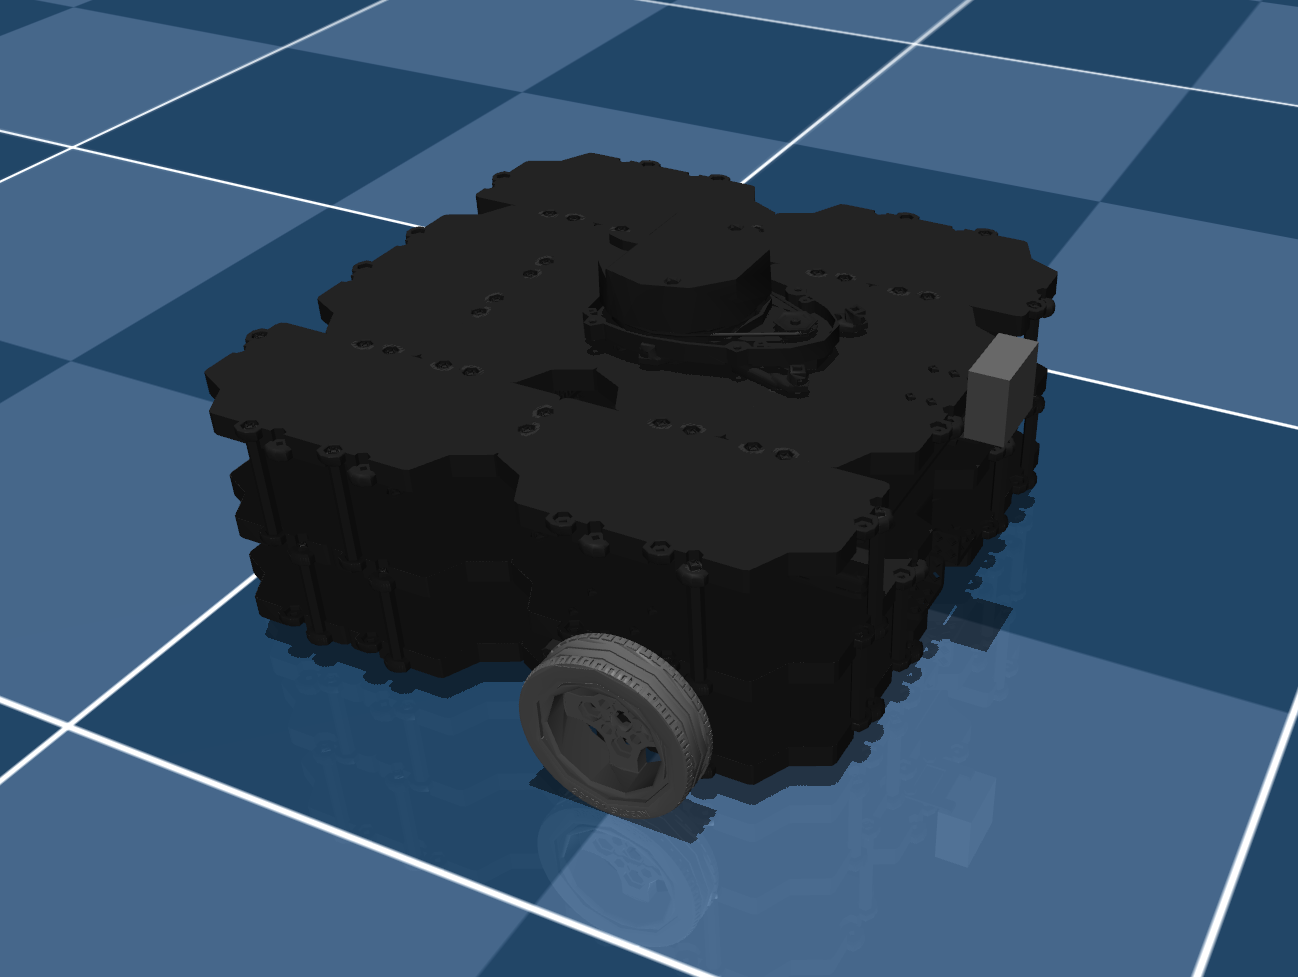
\includegraphics[width=\linewidth]{rrt_figures/turtlebot3_waffle_pi.png} \\
            \small \href{https://www.turtlebot.com/turtlebot3/}{\textit{TurtleBot3 Waffle Pi}}
        \end{column}
        \begin{column}{0.45\linewidth}
            \centering
            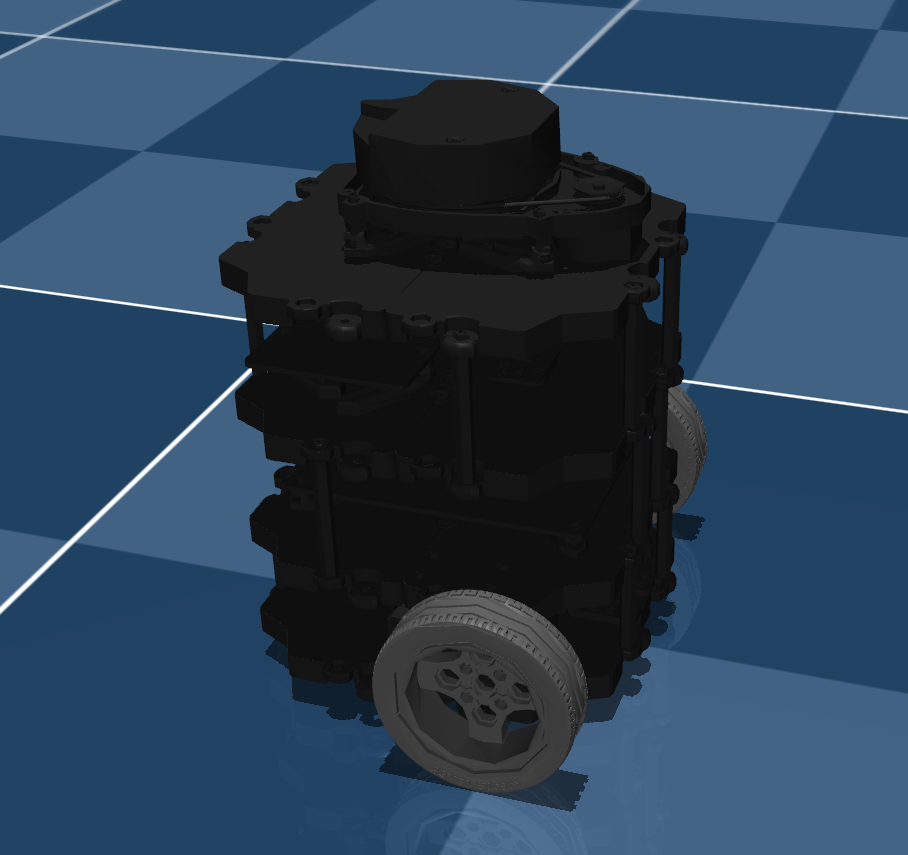
\includegraphics[width=\linewidth]{rrt_figures/turtlebot3_burger.png} \\
            \small \href{https://www.turtlebot.com/turtlebot3/}{\textit{TurtleBot3 Burger}}
        \end{column}
    \end{columns}
\end{frame}

\subsection{How it Works?}
\begin{frame}
    \frametitle{\insertsection \ - \insertsubsection}
    A \textbf{Differential Drive Robot} (DDR) is a type of mobile robot:
    \begin{enumerate}
        \item It moves on the 2D plane, and its state consists of its 2D position $(x, y)$ and its yaw angle orientation $\theta$:
              \[
                  \mathbf{x} = \begin{bmatrix} x & y & \theta \end{bmatrix}^\top \in \mathbb{R}^{3}
              \]
        \item It has \textbf{two independently actuated wheels} and usually another \textbf{one free turning supporting wheel}. Its motion is generated by the angular speeds $\omega_{L}$ and $\omega_{R}$ of its left and right wheel respectively.
        \item Important parameters affecting its motion are the \textit{fixed wheel distance} (separation) $\mathbf{L}$ and \textit{fixed wheel radius} $\mathbf{r}$.
        \item It is a \textbf{nonholonimic system}, obeying to an important motion constraint: \textbf{it can not move laterally} (sideways), assuming no slipping between the wheels and the ground. This is mathematically described by the Pfaffian nonholonomic constraint (on velocity):
              \[
                  \dot{x}\sin\theta - \dot{y}\cos\theta = 0 \Rightarrow
                  \begin{bmatrix} \sin\theta & -\cos\theta & 0 \end{bmatrix} \dot{\mathbf{x}} = 0
              \]
    \end{enumerate}
\end{frame}

\subsection{Kinematics of DDR}
\begin{frame}
    \frametitle{\insertsection \ - \insertsubsection}
    \begin{columns}
        \begin{column}{0.5\linewidth}
            \footnotesize
            For linear and angular velocities $v$, $\omega$ respectively of the DDR system, and wheel angular speeds $\omega_{L}$, $\omega_{R}$, we can derive the following state equations:
            \[
                \dot{\mathbf{x}} =
                \begin{bmatrix}
                    \cos\theta & 0 \\
                    \sin\theta & 0 \\
                    0          & 1
                \end{bmatrix} \cdot
                \begin{bmatrix}
                    v \\
                    \omega
                \end{bmatrix} =
                \begin{bmatrix}
                    \frac{r\cos\theta}{2} & \frac{r\cos\theta}{2} \\
                    \frac{r\sin\theta}{2} & \frac{r\sin\theta}{2} \\
                    -\frac{r}{L}          & \frac{r}{L}
                \end{bmatrix} \cdot
                \begin{bmatrix}
                    \omega_L \\
                    \omega_R
                \end{bmatrix}
            \]
            We can achieve desired velocities $v$, $\omega$, actuating the wheels with the following angular speeds $\omega_{L}$, $\omega_{R}$:
            \[
                \begin{aligned}
                    \begin{aligned}
                        v      & = \frac{r}{2}\left(\omega_R + \omega_L\right) \\
                        \omega & = \frac{r}{L}\left(\omega_R - \omega_L\right)
                    \end{aligned} \implies
                    \begin{aligned}
                        \omega_R & = \frac{1}{r}v + \frac{L}{2r}\omega \\
                        \omega_L & = \frac{1}{r}v - \frac{L}{2r}\omega
                    \end{aligned}
                \end{aligned}
            \]
        \end{column}
        \begin{column}{0.5\linewidth}
            \centering
            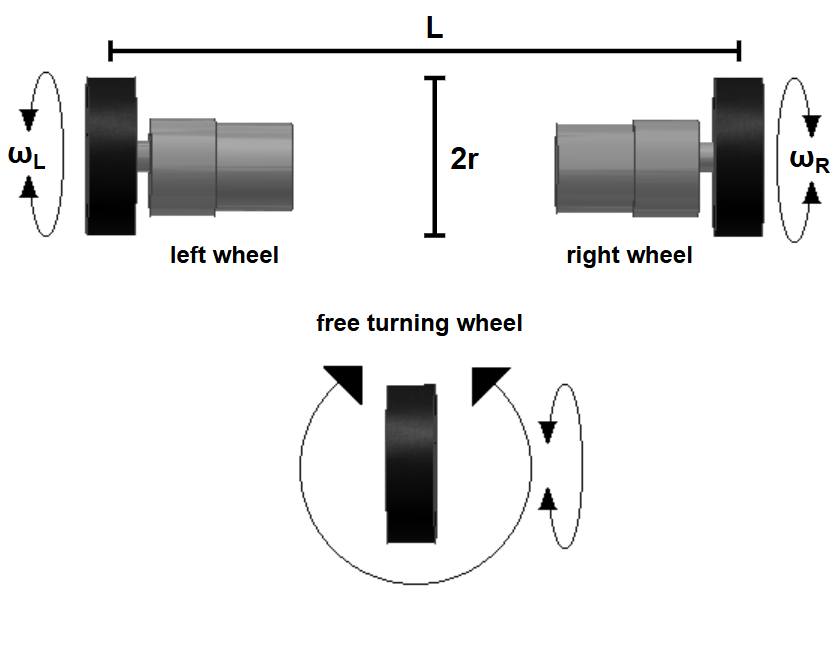
\includegraphics[width=\linewidth]{rrt_figures/differential_drive_system.png} \\
            \small \href{https://en.wikipedia.org/wiki/Differential_wheeled_robot}{\textit{Differential Drive System Diagram}}
        \end{column}
    \end{columns}
\end{frame}

\subsection{Other Wheeled Robots}
\begin{frame}
    \frametitle{\insertsection \ - \insertsubsection}
    \begin{columns}
        \begin{column}{0.5\linewidth}
            \textbf{Holonomic robots}
            \begin{itemize}
                \item Omnidirectional (mecanum) wheels
                \item Can move in any direction instantly (no velocity constraint)
            \end{itemize}
            \textbf{Car-like robots}
            \begin{itemize}
                \item Ackermann steering
                \item Turning radius constraint
            \end{itemize}
            \vspace{10pt}
            The type of mobile robots we use here, \textbf{differential drive} ones, are:
            \begin{itemize}
                \item Simple
                \item Cheap
                \item Very common in research
            \end{itemize}
        \end{column}
        \begin{column}{0.5\linewidth}
            \centering
            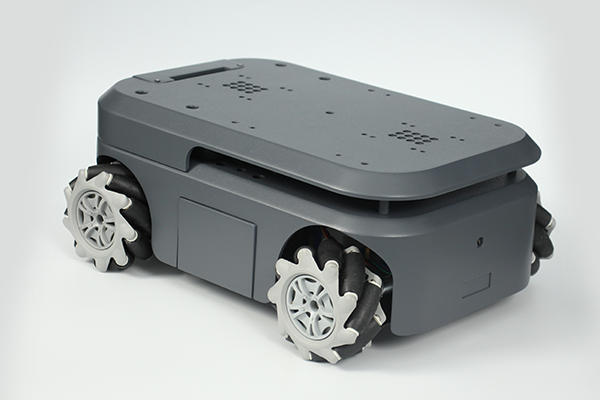
\includegraphics[width=\linewidth]{rrt_figures/myAGV_elephant.png} \\
            \small \href{https://www.elephantrobotics.com/en/myagv-new-en/}{\textit{MyAGV Elephant Robotics (omnidirectional)}}
        \end{column}
    \end{columns}
\end{frame}

\addtocontents{toc}{\vskip 10pt}

% Rapidly-exploring Random Tree (RRT)
\section{Rapidly-exploring Random Tree (RRT)}

\subsection{What it is \& Properties}
\begin{frame}
    \frametitle{\insertsection \ - \insertsubsection}
    \textbf{RRT} (Rapidly-exploring Random Tree) is a \textbf{probabilistic} algorithm designed for efficient \textbf{path planning} in \textit{high-dimensional}, \textit{complex}, and \textit{continuous spaces}, commonly used in robotics for \textbf{motion planning}. It works by building a \textbf{tree} from a start point, expanding toward \textbf{random samples}, and \textbf{checking for collisions} in the process.
    \vspace{5pt}
    \begin{enumerate}
        \item Purpose:
              \begin{itemize}
                  \item Find a \textbf{collision-free path} in continuous, complex geometries.
                  \item Work in the continuous state space, \textbf{without explicit environment decomposition} (e.g., grid discretization, cell decomposition).
              \end{itemize}
        \item Key Properties:
              \begin{itemize}
                  \item \textbf{Probabilistically complete} (finds a solution if one exists). It is guaranteed to converge to a \textbf{feasible solution} (given enough time), which is generally \textbf{not path-optimal, nor control-optimal}. For optimality (at least asymptotic) there is RRT*.
                  \item \textbf{Naturally explores} large unexplored regions.
                  \item \textbf{Easy to implement} in a large variety of systems.
              \end{itemize}
    \end{enumerate}
\end{frame}

\subsection{Algorithm Description}
\begin{frame}
    \frametitle{\insertsection \ - \insertsubsection}
    \begin{columns}
        \begin{column}{0.5\linewidth}
            \footnotesize
            Assume state space $X$, free space $X_{free} \subseteq X$, and obstacle space $X_{obs} = X \setminus X_{free}$. RRT builds a tree incrementally, initializing the search from the node $\mathbf{x}_{start} \in X_{free}$ and then iteratively:
            \begin{enumerate}
                \item Sample random state $\mathbf{x}_{sample} \in X$
                \item Find nearest node $\mathbf{x}_{near} \in X_{free}$ to $\mathbf{x}_{sample}$ according to a distance metric
                \item Steer toward sample (up to a fixed step size) and get a potential new node $\mathbf{x}_{new} \in X$
                \item Check for collisions and add the new node only if $\mathbf{x}_{new} \notin X_{obs}$
            \end{enumerate}
            Stop when goal $\mathbf{x}_{goal} \in X_{free}$ is reached, and retrieve feasible path from the parent nodes using backtracking.
        \end{column}
        \begin{column}{0.5\linewidth}
            \centering
            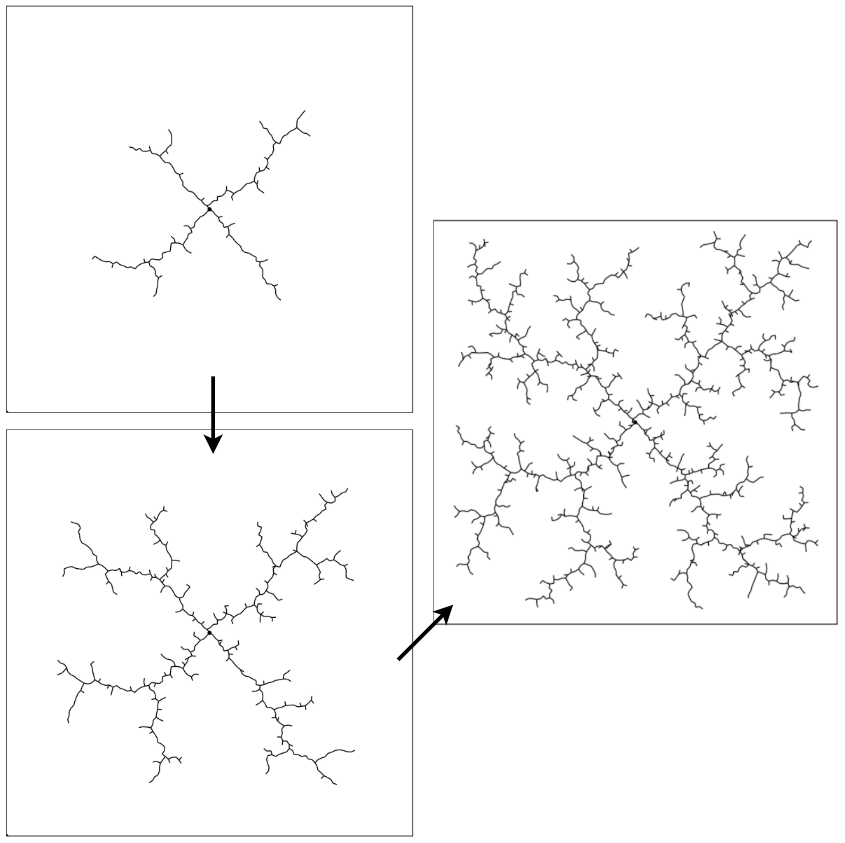
\includegraphics[width=\linewidth]{rrt_figures/rrt_expansion.png} \\
            \small \href{https://msl.cs.illinois.edu/~lavalle/papers/Lav98c.pdf}{\textit{RRT expansion example}}
        \end{column}
    \end{columns}
\end{frame}

\addtocontents{toc}{\vskip 10pt}

% Prim's Algorithm
\section{Prim's Algorithm}

\subsection{What it is \& Properties}
\begin{frame}
    \frametitle{\insertsection \ - \insertsubsection}
    \textbf{Prim's algorithm} is a \textbf{greedy} algorithm for constructing a \textbf{Minimum Spanning Tree (MST)} of a \textbf{weighted, undirected graph}. It starts from an arbitrary start node and incrementally builds a \textbf{tree/subgraph} by repeatedly adding the \textbf{minimum weight edge} that connects a new vertex to the growing tree/subgraph.
    \vspace{5pt}
    \begin{enumerate}
        \item Purpose:
              \begin{itemize}
                  \item Construct a \textbf{Minimum Spanning Tree (MST)}, by connecting all vertices with the \textbf{minimum possible total edge weight}.
              \end{itemize}
        \item Key Properties:
              \begin{itemize}
                  \item \textbf{Greedy algorithm} (similar in spirit to Kruskal’s algorithm).
                  \item Produces a \textbf{fully connected}, \textbf{acyclic}, and \textbf{undirected} graph (the MST, which is a subgraph of the original graph).
                  \item Resulting structure contains exactly $|E|=|V|-1$ edges, where $|V|$ is the number of vertices.
              \end{itemize}
    \end{enumerate}
\end{frame}

\subsection{Algorithm Description}
\begin{frame}
    \frametitle{\insertsection \ - \insertsubsection}
    \begin{columns}
        \begin{column}{0.5\linewidth}
            \footnotesize
            Steps of Prim's algorithm:
            \begin{enumerate}
                \item Start from an arbitrary vertex
                \item Mark it as part of the MST
                \item Add all edges from this vertex to a candidate edge list
                \item While candidate list is not empty:
                      \begin{itemize}
                          \item Select edge with minimum weight (if more than one choose randomly)
                          \item Remove the selected edge from the candidate list
                          \item If the edge connects to a vertex not in MST, add that vertex to MST and add its outgoing edges to the candidate list
                      \end{itemize}
            \end{enumerate}
            Continue until all vertices are included in the Minimum Spanning Tree (MST).
        \end{column}
        \begin{column}{0.5\linewidth}
            \centering
            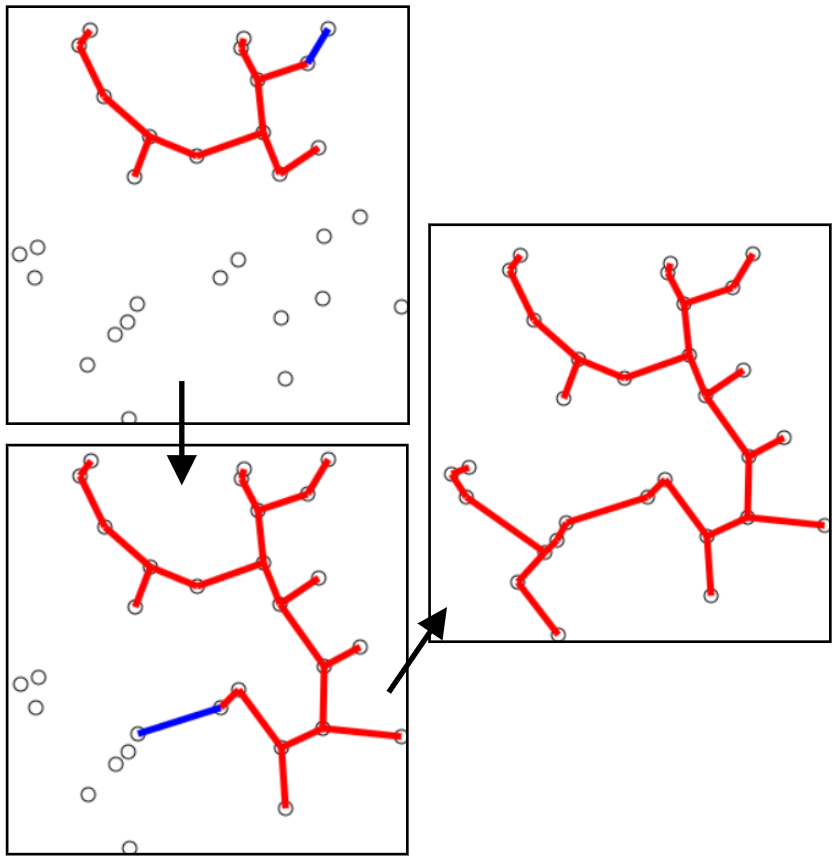
\includegraphics[width=\linewidth]{rrt_figures/prim_algorithm_MST.png} \\[0.3em]
            \small \href{https://en.wikipedia.org/wiki/Prims_algorithm}{\textit{Prim's algorithm MST example}}
        \end{column}
    \end{columns}
\end{frame}

\addtocontents{toc}{\vskip 5pt}

% Exercise
\section{Maze Exercise in MuJoCo}
\begin{frame}
    \frametitle{\insertsection}
    \begin{columns}
        \begin{column}{0.45\linewidth}
            \centering
            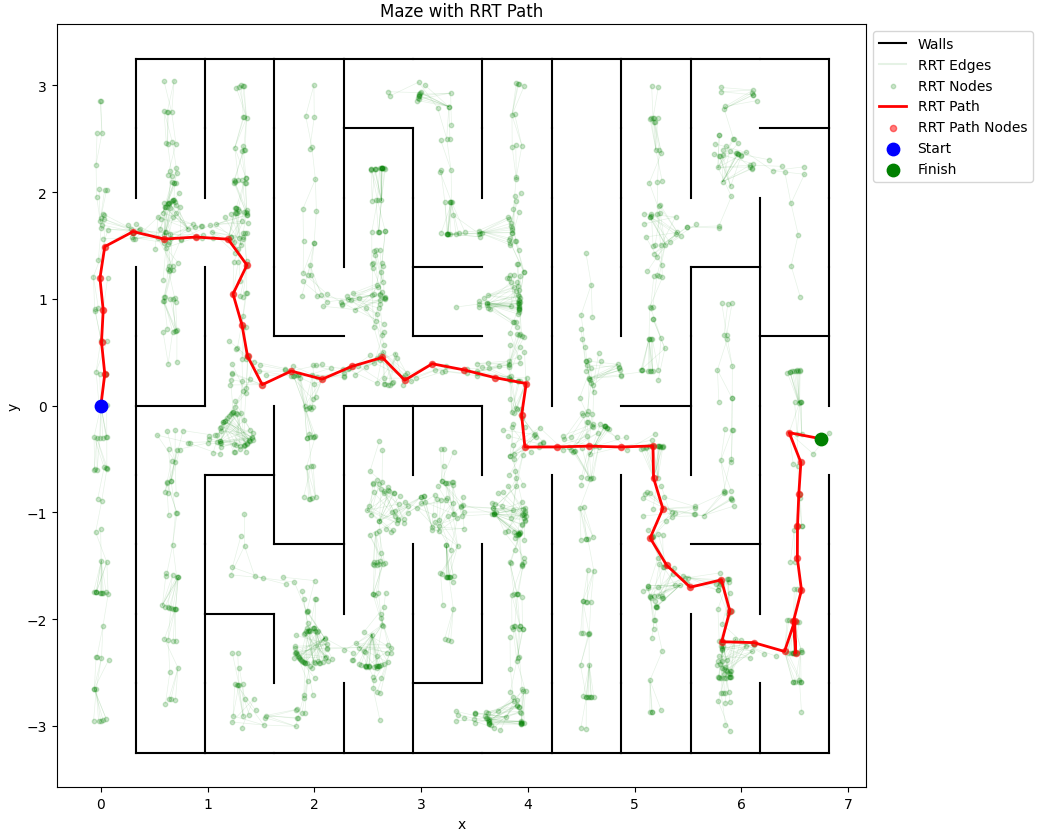
\includegraphics[width=\linewidth]{rrt_figures/maze_RRT_plot.png} \\
            \small \textit{Solving Maze using RRT}
        \end{column}
        \begin{column}{0.55\linewidth}
            \centering
            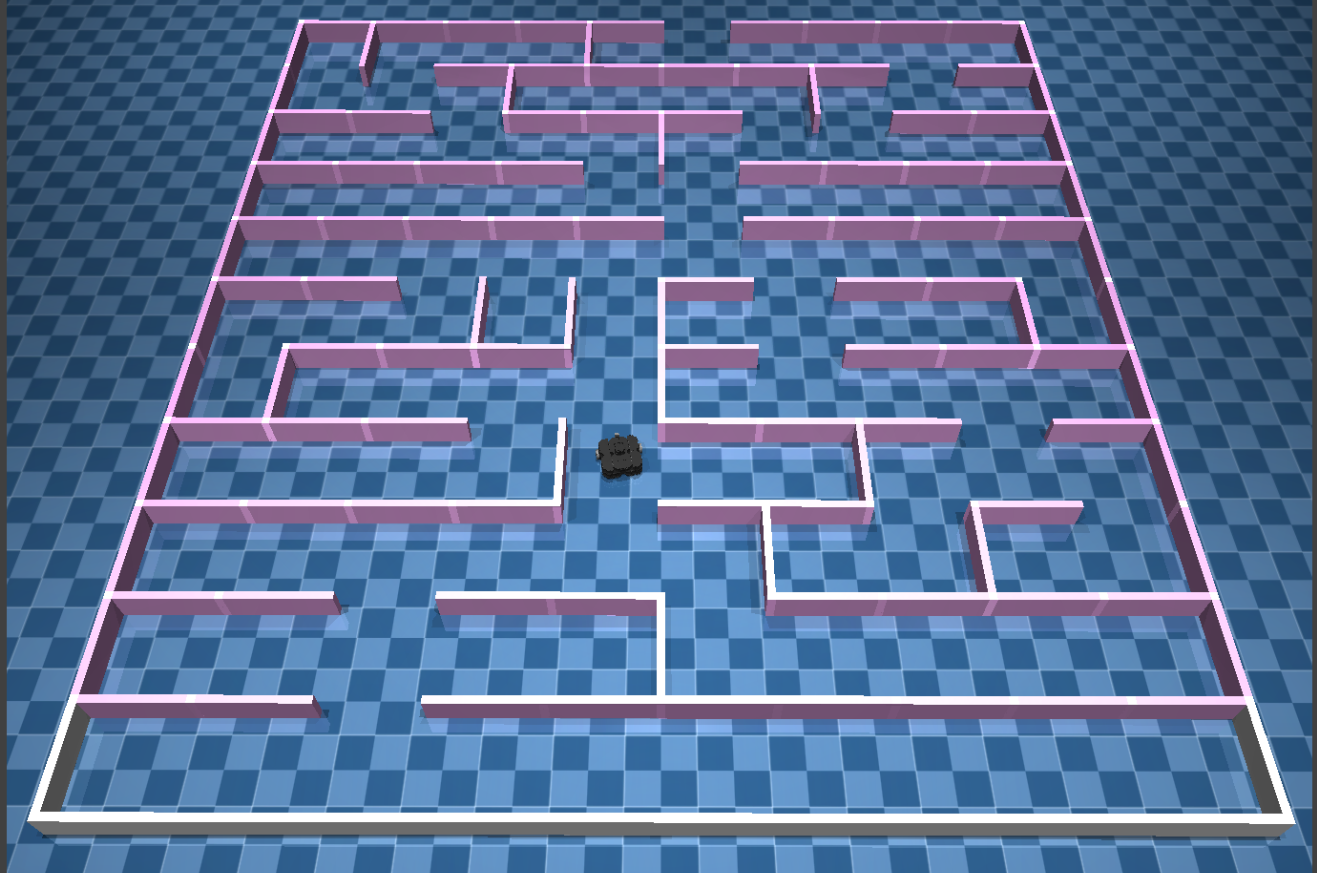
\includegraphics[width=\linewidth]{rrt_figures/maze_solve_mujoco.png} \\
            \small \textit{Maze and Bot View in MuJoCo}
        \end{column}
    \end{columns}
\end{frame}

\subsection{Constructing Random Mazes}
\begin{frame}
    \frametitle{\insertsection \ - \insertsubsection}
    We use a \textbf{randomized version of Prim's algorithm} for maze generation.
    \vspace{5pt}
    \begin{enumerate}
        \item Graph Interpretation:
              \begin{itemize}
                  \item \textit{Cells} $\leftrightarrow$ \textit{Nodes}
                  \item \textit{Walls} $\leftrightarrow$ \textit{Edges}
                  \item \textit{Removing a wall} $\leftrightarrow$ \textit{Adding an edge} to the spanning tree
              \end{itemize}
        \item Randomized Prim Variant:
              \begin{itemize}
                  \item We assume all edges have \textbf{equal cost}.
                  \item \textbf{No minimum-weight edge comparison} is required.
                  \item The next edge is chosen applying a \textbf{weighted random selection}. We assign directional probabilities/biases $P_{N}$ (North), $P_{S}$ (South), $P_{E}$ (East), $P_{W}$ (West), for which $P_{N} + P_{S} + P_{E} + P_{W} = 1$. So, if for example $P_{N} + P_{S} > P_{E} + P_{W}$, then there is a higher vertical direction probability, which results to longer vertical corridors in the maze.
              \end{itemize}
    \end{enumerate}
    \vspace{5pt}
    Prim's algorithm generates a \textbf{perfect maze}, meaning that it has exactly one \textbf{unique path between any two cells}, with \textbf{no loops or inaccessible areas}.
\end{frame}

\begin{frame}
    \frametitle{\insertsection \ - \insertsubsection}
    \centering
    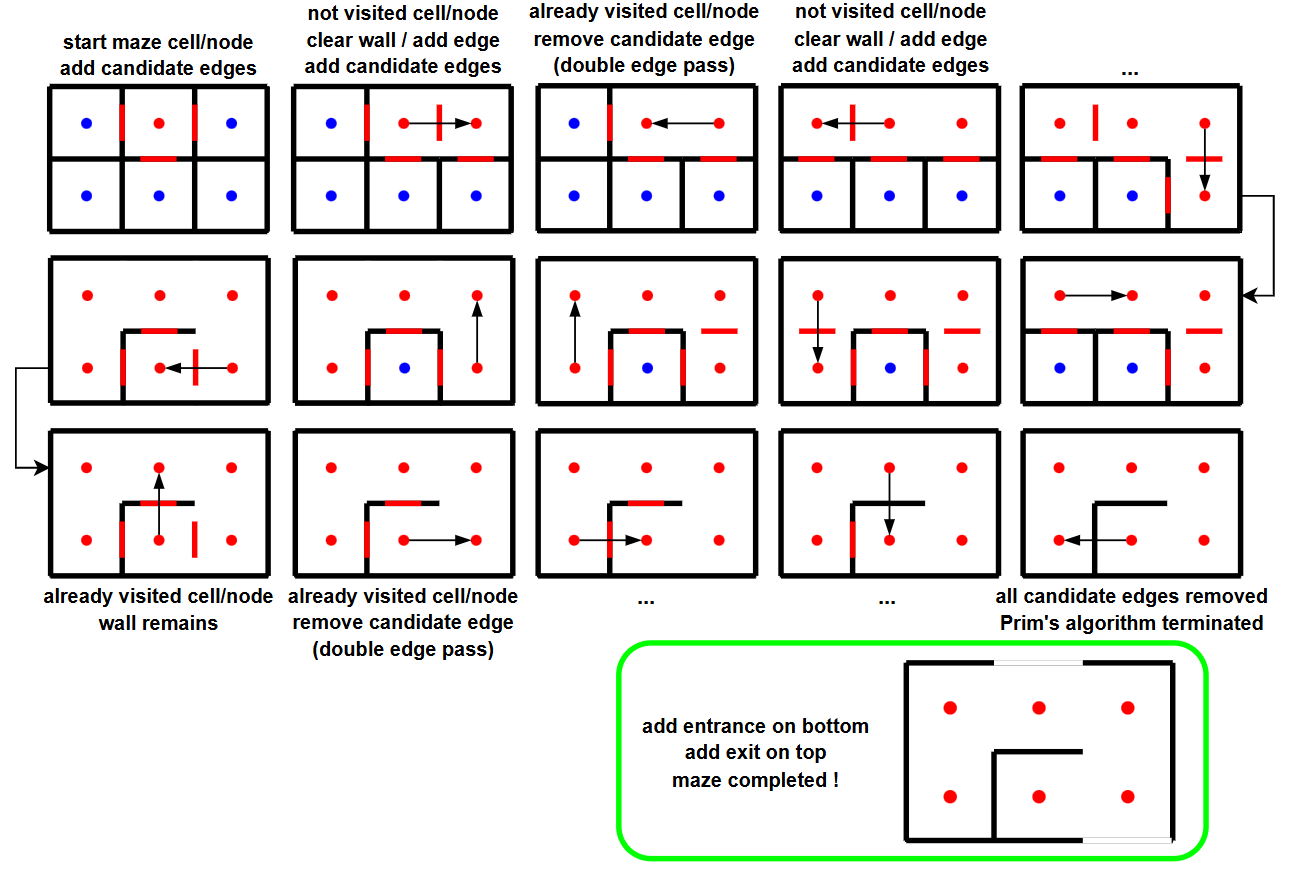
\includegraphics[width=0.9\linewidth]{rrt_figures/maze_construction_steps_example.png} \\
    \small \textit{Construction steps of a $2\times3$ maze. Blue and red cells represent the unvisited and visited nodes respectively. Red walls represent the candidate edges left.}
\end{frame}

\begin{frame}
    \frametitle{\insertsection \ - \insertsubsection}
    \begin{columns}
        \begin{column}{0.4\linewidth}
            \footnotesize
            Mazes are constructed using a randomized version of Prim's algorithm. Some parameters to experiment with are:
            \begin{itemize}
                \item number of \textbf{rows} \& \textbf{columns}
                \item \textbf{directional probabilities} for Prim's algorithm
                \item \textbf{wall thickness}
                \item \textbf{RNG seed}
                      \vspace{5pt}
                \item \textit{cell size} (wall length)
                \item \textit{position} and \textit{orientation} of maze on 2D plane
            \end{itemize}
            \vspace{5pt}
            Mazes are exported to:
            \begin{itemize}
                \item \textbf{Real Dimensions} XML
                \item \textbf{Inflated-Walls} XML for RRT
            \end{itemize}
        \end{column}
        \begin{column}{0.6\linewidth}
            \centering
            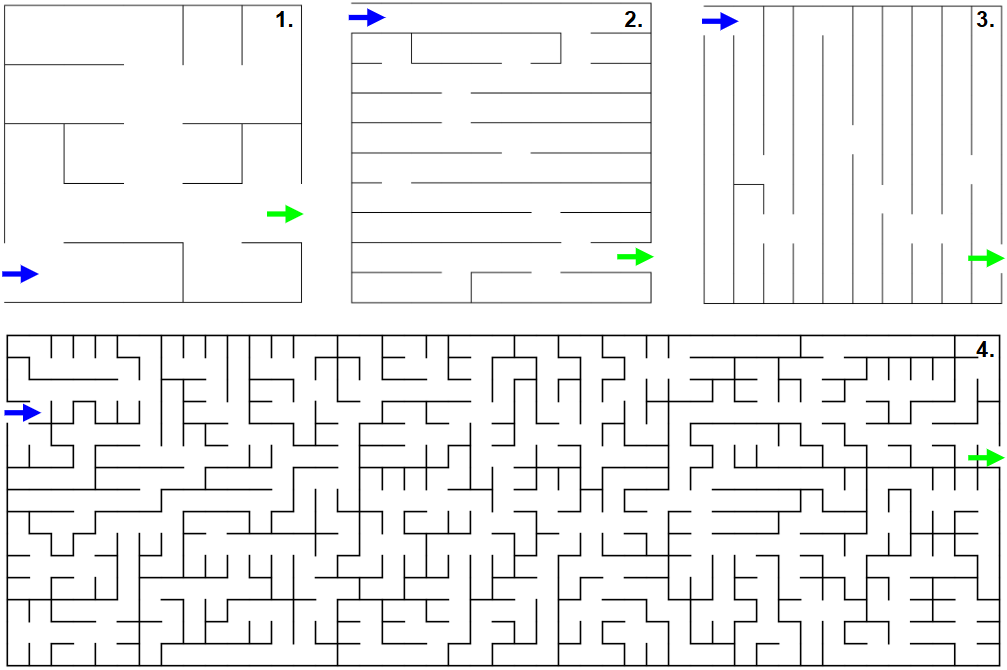
\includegraphics[width=\linewidth]{rrt_figures/mazes_examples.png} \\
            \small \textit{Random Mazes examples, with a single entrance and a single exit}
        \end{column}
    \end{columns}
\end{frame}

\begin{frame}
    \frametitle{\insertsection \ - \insertsubsection}
    \centering
    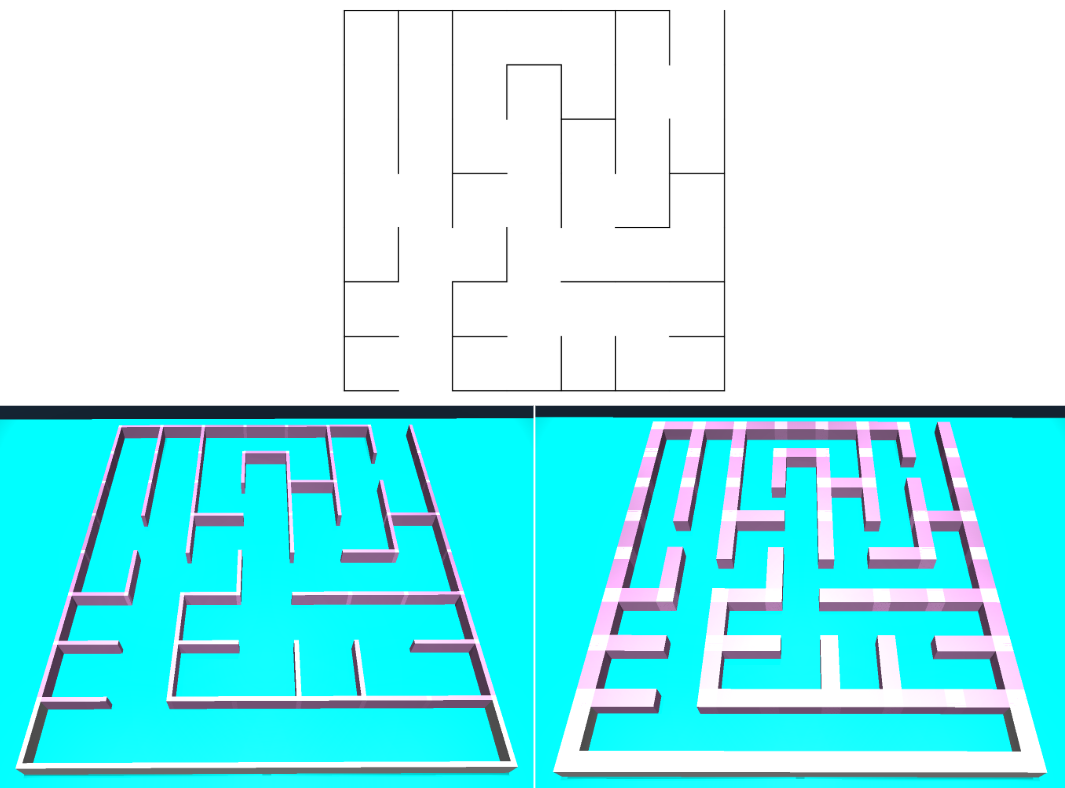
\includegraphics[width=0.8\linewidth]{rrt_figures/maze_real_inflated_example.png} \\
    \small \textit{Comparison between real dimensions maze and inflated maze in MuJoCo view.}
\end{frame}

\subsection{Path Planning using RRT}
\begin{frame}
    \frametitle{\insertsection \ - \insertsubsection}
    \begin{enumerate}
        \item \textbf{Assumptions:}
              \begin{itemize}
                  \item \textbf{\textit{Known} maze structure} and \textbf{robot state} (via MuJoCo).
                  \item LiDAR (or any other sensor) not used for state estimation.
              \end{itemize}
              \vspace{5pt}
        \item \textbf{Planning in} $\mathbf{SE(2)}$:
              \begin{itemize}
                  \item State space: $\mathbf{x} = \begin{bmatrix} x & y & \theta \end{bmatrix}^\top \in \mathbb{R}^{3}$.
                  \item \textbf{Weighted distance} metric: $d^2 = dx^2 + dy^2 + w_\theta(d\theta)^2$.
                  \item \textbf{Goal sampling bias} and \textbf{search area sampling asymmetry} applied.
              \end{itemize}
              \vspace{5pt}
        \item \textbf{Collision Checking (Physics-Based):}
              \begin{itemize}
                  \item Use \textbf{inflated walls}.
                  \item \textbf{Discretize candidate edge}, set robot pose iteratively for every interpolated point, and run the system forward. If any \textit{contact} is detected between the mobile robot and the walls, \textit{reject the edge}.
              \end{itemize}
              \vspace{5pt}
        \item \textbf{Execution Phase:}
              \begin{itemize}
                  \item Load real maze and \textit{follow RRT path} using a \textbf{cascaded P-controller}.
                  \item \textbf{Goal condition} (RRT termination condition):
                        \[
                            \|p - p_{goal}\| < \epsilon_{xy}, \quad
                            |\theta - \theta_{goal}| < \epsilon_\theta
                        \]
              \end{itemize}
    \end{enumerate}
\end{frame}

\begin{frame}
    \frametitle{\insertsection \ - \insertsubsection}
    \centering
    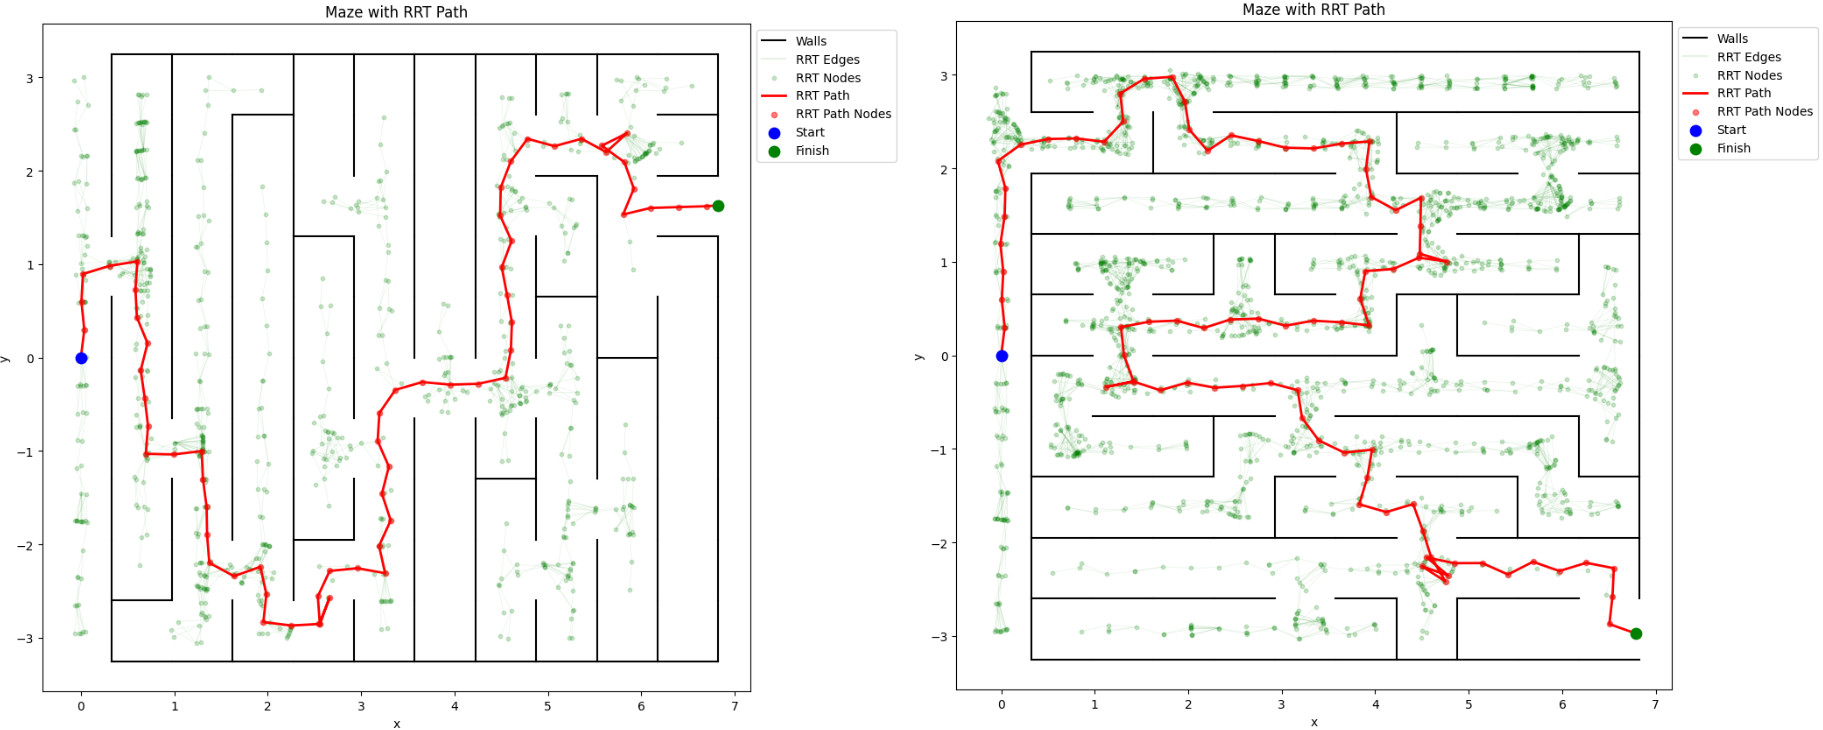
\includegraphics[width=\linewidth]{rrt_figures/maze_RRT_plots_examples.png} \\
    \small \textit{Solving mazes using RRTs. First found feasible paths are shown, along with all the RRT nodes and edges.}
\end{frame}

\subsection{Full Example}
\begin{frame}
    \frametitle{\insertsection \ - \insertsubsection}
    \centering
    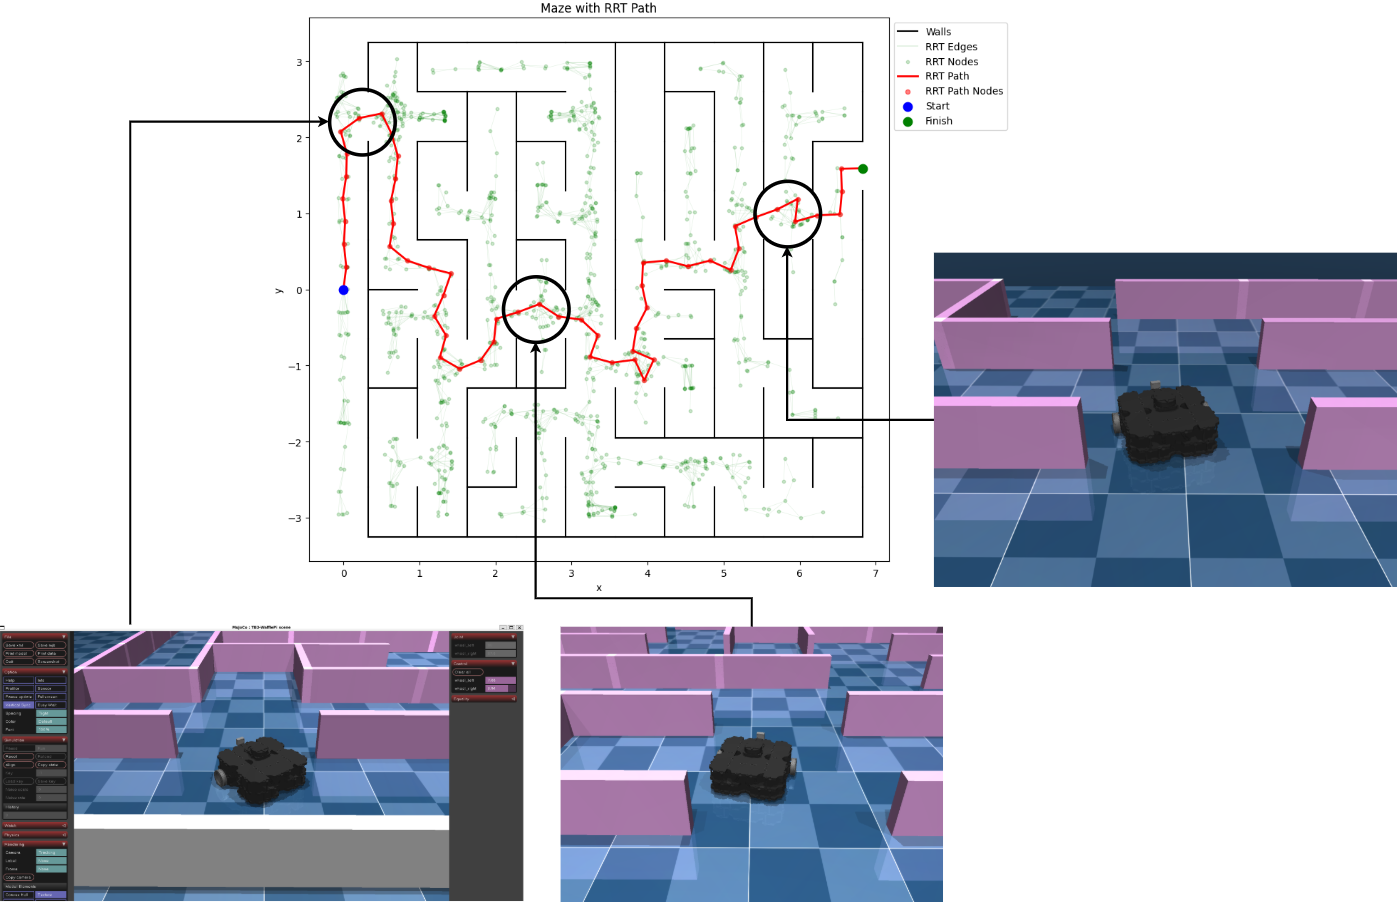
\includegraphics[width=0.9\linewidth]{rrt_figures/maze_solve_full_example.png} \\
    \small \textit{Full example shown, with the found feasible RRT path from start to finish, and MuJoCo view frames from key points inside the maze}
\end{frame}

\subsection{Handling MuJoCo Environment}
\begin{frame}
    \frametitle{\insertsection \ - \insertsubsection}
    \centering
    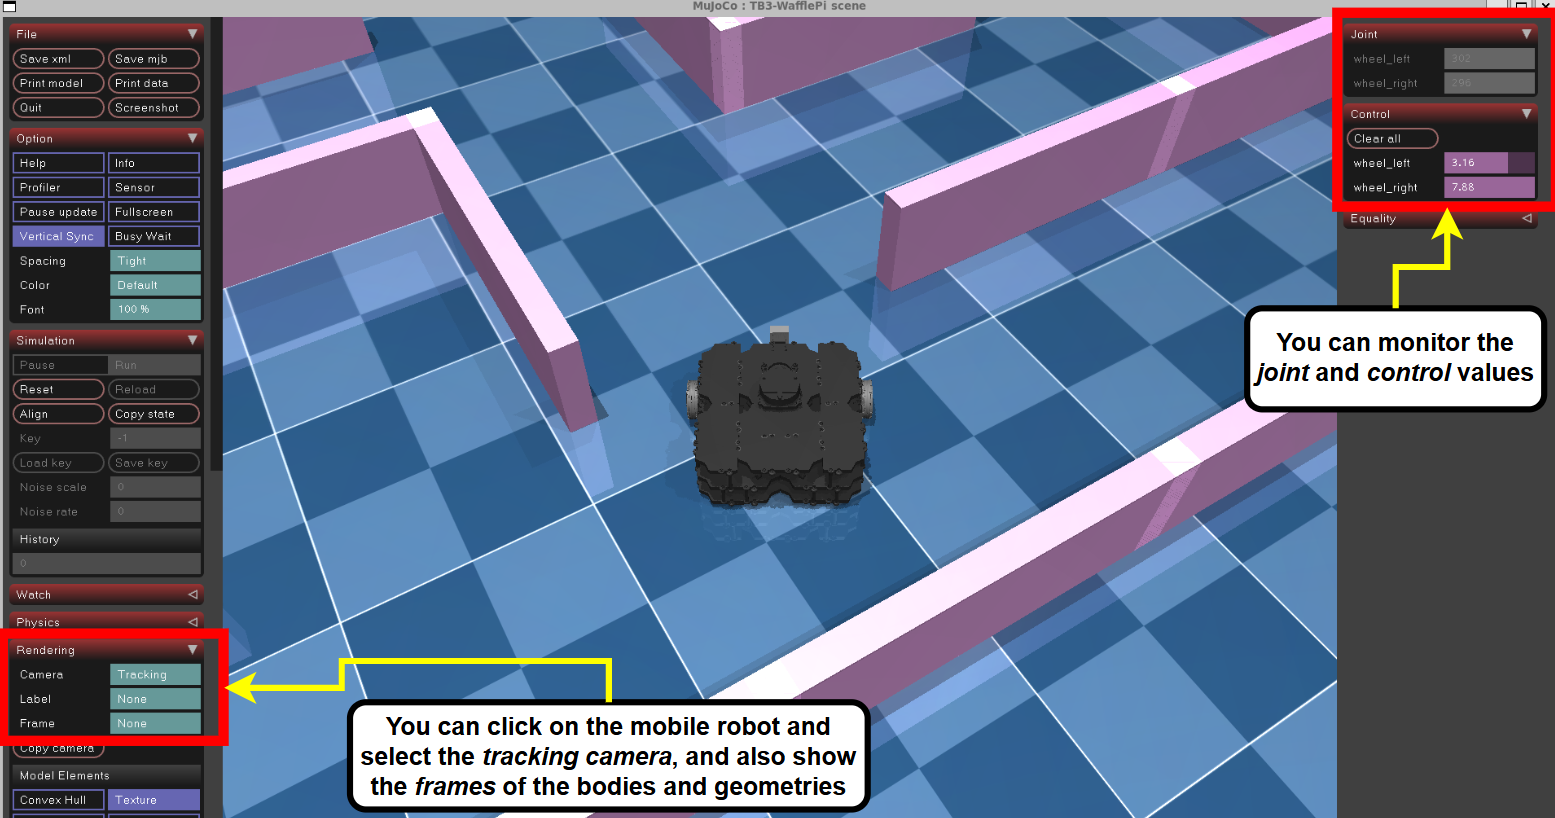
\includegraphics[width=\linewidth]{rrt_figures/mujoco_environment.png} \\
    \small \textit{Showing some MuJoCo utilities}
\end{frame}

\addtocontents{toc}{\vskip 5pt}

% References
\section{References}
\begin{frame}{\insertsection}
    \begin{itemize}
        \item \href{https://en.wikipedia.org/wiki/Differential_wheeled_robot}{\textbf{Differential Drive Robot basic info}}
        \item \href{https://msl.cs.illinois.edu/~lavalle/papers/Lav98c.pdf}{\textbf{RRT original paper "Rapidly-Exploring Random Trees: A New Tool for Path Planning"}}
        \item \textbf{Other RRT sources:} \href{https://en.wikipedia.org/wiki/Rapidly_exploring_random_tree}{\textbf{source1}} \textbf{\&} \href{https://theclassytim.medium.com/robotic-path-planning-rrt-and-rrt-212319121378}{\textbf{source2}}
        \item \textbf{Prim's algorithm} \href{\detokenize{https://en.wikipedia.org/wiki/Prims_algorithm}}{\textbf{source1}} \textbf{\&} \href{https://www.geeksforgeeks.org/dsa/prims-minimum-spanning-tree-mst-greedy-algo-5/}{\textbf{source2}}
        \item \href{https://mujoco.readthedocs.io/en/stable/overview.html}{\textbf{MuJoCo documentation}}
        \item \href{https://github.com/google-deepmind/mujoco_menagerie}{\textbf{A collection of high-quality models for the MuJoCo physics engine, curated by Google DeepMind (MuJoCo Menagerie)}}
        \item \href{https://hades.mech.northwestern.edu/images/7/7f/MR.pdf}{\textbf{Modern Robotics: Mechanics, Planning, and Control; Kevin M. Lynch and Frank C. Park}}
    \end{itemize}
\end{frame}

\end{document}
